\section{Literature Review}
% Review of previous works, e.g. previous papers:
% Review of State of the Art (SotA), e.g. existing/related implementations:

% Need a quick intro?
% Within this section we shall outline and review related works and prior studies to support the development of our proposed system.\\
% This will cover a review of studies into 

% Include Comments on what will be taken from prior works for our current work
% What will we try differently?

%% Lit Review

% Interaction With The Head
% |- Devices Generally
% |- Spacial Vs Semantic Vs Natural Input
% |- Mobile devices
%    |- One-handed interaction
% 3D interfaces
% |- Viewed on 2D screen
% |- Reactive to user's head vs phone
% Summary of Relationship between head and phone (how tracked/detected)

% Related works
% [ ] Thumb Reachability on Mobile Devices ???
%       Quick summary/review of using phone with modern screen sizes | Find References on any studies
%       just a paragraph or two to back-up claim in the intro, unless covered 

% [ ] Head Gestures / Control
%  |- Head gestures generally (not specific to mobile devices) | Find References
%  |  |- Head Controls With Mobile Devices | Already Have plenty of references
%  |     |- One-handed & Hands-Free interaction
%  |- Head Tracking Techniques (From Special hardware to camera only) | Find References
%  |- Types of Gesture (Semantic Vs Spatial) and Examples | Find References
  
% [ ] Adaptive Interfaces
%  |- 3D Interfaces (AR/VR) | Find References
%  |   |- Having additional content off-screen that can be accessed by changing perspective
%  |   |- Responsive to phone movement vs head movement | Find References
%  |- Context Aware UI | Find References
%     |- Reactive to user context to adjust on screen elements
%     |- Reactive to head/gaze?


% Look at https://faculty.washington.edu/wobbrock/pubs/Wobbrock-2015.pdf

% Intro into the section?
%   Need to describe what this will do, or just say discussing related works / further exploring works described in the intro?

% \subsection{Smartphone Usability}
% Reachability, comfort, relationship to screensize, typical input modalities
% Further review into why want to develop this system?

% How to intro?
% Tie directly to screen-size?

% Screen-size is growing (not for all models of all brands, but screen sizes are definitely larger than previously)
% screen-size tied to phone usability 
% one-handed interaction? Or simply note that one of the avenues within which screen-size is a factor is one-handed use (people use both).

% \cite{xuesheng2018research} Modern mobile device screens getting larger (when reviewing the largest market-share smartphone brands worldwide (at the time of writing), Samsung and Apple)


% \cite{tsai2017testing} Review usability of touch-screens of different size, though mainly age-groups

% \cite{le2018fingers} Study with 4 phones with increasing screen size, investigating the areas of the screen which are obtainable with each digit (Screen for thumb, phone back for fingers)\\
% As expected, larger screen sizes afforded less coverage for the thumb, in-particular reaching the upper parts of the screen, and in some-cases the side of the screen opposite to the thumb\\
% However this study did not ensure grip was consistent between participants, or that participants keep a constant grip. As such it isn't clear if some observed reachability is due to grip, hand-size, or adjusted grips.\\

% \cite{punchoojit2017usability} Usability of phone generally, touches on touch screens

% \cite{raptis2013does} Usability with respect to touch-screen

% \cite{williamson2011multimodal} evaluation of touch gestures on screen

\subsection{Head Gestures}
% Examples of head gestures

% Start with tracking that requires specific tech, e.g. AR / VR, or say TiltCap, require head-mounted/earable or special camera (IR)
% Can start to refine to camera/webcam only, particularly ML based approaches and worth mentioning haar/harr cascades to identify faces quickly
% Maybe mention motion correlation as way to track lateral movement of something

% \subsubsection{Head Tracking Techniques} % Ideally explain tracking type in evaluation, e.g. needing additional hardware / software in the evaluation of the system, alongside the actual gestures

% Review of head gestures / study?
% Gestures as form of control
\cite{rudigkeit2015analytical} usage of an IMU, within a headband on a user's head, to track pitch and roll (nodding up/down and left/right) of the head.\\
Performed by tracking the changes in linear acceleration (why not angular?) detected by the IMU along the Pitch and Yaw degrees of freedom.
These were used to detect nodding left, right, up, and down.\\
To avoid tracking involuntary / small head movements, a low-pass filter was applied to the IMU output.
To improve gesture recognition for specific users, they are able to customise parameters of the model, such as minimum thresholds of movement (for the low-pass filter), maximum displacement (to avoid when user is going beyond range for gesture), time window (how quickly a nod need be performed for the action).\\
Of the 10 participant, 9 achieved greater than 80\% classification rate using the globally tuned model params, with all being able to achieve equal or better accuracy with individually tuned parameters.
Used to perform motions with a robotic arm (e.g. lateral movements in a given plane, or rotations). Plane actions performed on switched via additional input, not gestures.
% Further reviewed by jackowski2017head

\cite{hachaj2019evaluation} Also utilises IMU from within a VR head-set. 
Compares several techniques, Principal Component Analysis (PCA, classification based on identifying the most 'important' feature and classifying on that feature), Dynamic Time Warping (DTW, computing the similarity between observed motion and gesture classes), Neural Networks (NN), and Random Forests.
Gesture set was simple, nodding, looking left / right.
Extracted gestures not used

\cite{yan2018headgesture} Propose several gestures for specific actions using IMU on a hololens to interact with display, seen in \autoref{fig:yan2018headgesture_proposed_gestures}\\
\begin{figure}
    \centering
    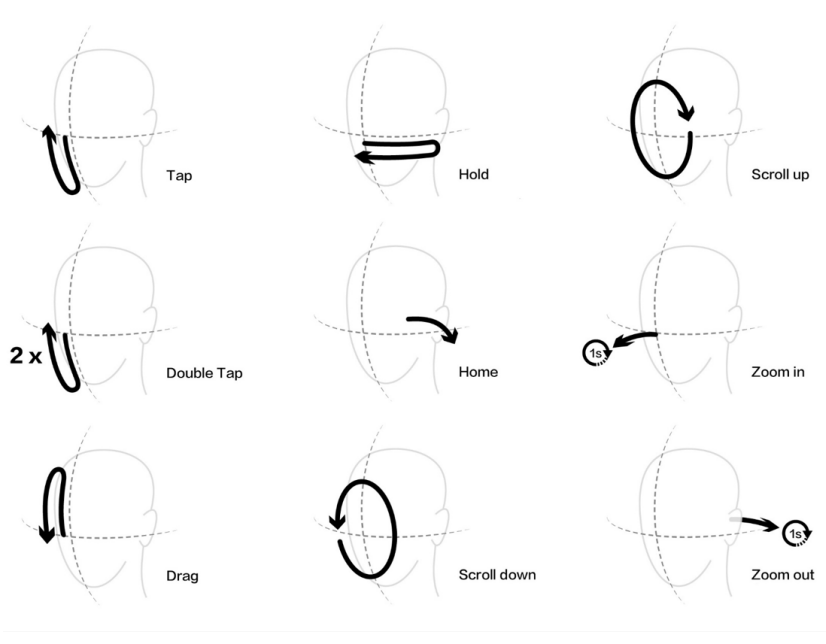
\includegraphics[width=0.5\textwidth]{figures/yan2018headgesture_fig2_proposed_gestures.png}
    \caption{\label{fig:yan2018headgesture_proposed_gestures} Proposed head gestures and their corresponding actions (p10)\cite{yan2018headgesture}}
\end{figure}
gestures segmented via detection of acceleration (20 Degrees per second) and deceleration (4 Degrees per second), not exceeding 2 seconds.\\
Feature extraction performed with DTW (same approach as evaluated by \cite{hachaj2019evaluation}), followed by an SVM classifier to classify the observed gesture into one of 9 categories, or unintentional movement.\\
Compared head gestures with hand gestures. Found that head gestures caused more fatigue and generally felt less natural, however were similar / slightly better with regards to learning effort

% Gestures as interface interactions
% Closer to mobile, as have just reliance on cameras
\cite{gorodnichy2002importance}, using a single camera. Feature defined by intensity gradient (e.g. change in lighting/colour, such as corners). Since nose is always closest to the camera, and convex in nature, it should be the 'brightest' feature. The tracked point isn't a specific point on the nose (e.g. the tip), but a point that can move across the surface of the nose, based on what is closest to the camera.\\
They go on to extend this work with \cite{gorodnichy2004nouse} Usage of the user's nose to control a pointer on their screen\\
Usage of nose to meet requirements for trackable feature that is always visible (presuming the user is facing within 180 degrees towards the camera)\\
Utilises stereography (e.g. 2 cameras) to perform the tracking, each with resolution as little as 160x120px
For accuracy/fidelity the system also requires 2 additional features of the face to track, with relation to the nose.\\
To click with the 'Nouse' the user blinking twice within short succession. Determined by reviewing the change in the sequence of 3 frames.\\
Low resolution to permit real-time tracking.\\
Cursor utilised to play pong, draw, and adjust pose of 3D model.\\
They make claims about accuracy and enjoyment, but relevant data not provided, just statements made suggesting Nouse was as good / if not better than typical mouse control (claim mouse causes wrist ache, but movement of entire head doesn't present neck ache?)
% No machine learning

\cite{varona2008hands} another nose based control, however uses Haar cascades to perform face-detection, within which they use a similar technique as \cite{gorodnichy2002importance} to extract points for the corners of the nose, or the nostrils.\\
Segment face region into 3 sections, eyes/eyebrows, nose, and mouth.\\
To detect eyes, determine user's skin colour by sampling the pixels within the detected face region. They then presume the eyes will be a different colour, and as such filter based on the extracted skin-tone. They then select the features closest to the nose, that are symmetrical.\\
With the features they use the nose to infer direction and velocity of the cursor. For mouse buttons, a UI is created with the actions as buttons. User moves cursor to the action tye wish to perform, then wink (with either eye) to select it. When they then fixate on part of the screen (move the cursor to a point and keep it stationary), the action will be performed.\\
Only evaluated for click recognition and accuracy of where the click was performed within a grid of points. However >80\% accuracy even for users with no training time, just instructions.\\
Not compared to usage of a mouse, however was designed for those who could not use a mouse, or might find it difficult.

\cite{saikia2013head} Usage of optical flow to extract the motion of the user's head.\\
Background subtraction performed with Gaussian Mixture Models. Effectively classifying pixels based on probability that they belong to user, which can be adjusted ont he fly to adapt to slowly changing light levels and changes to elements of the background.\\ % understand a bit more before submission
Optical Flow techniques then used to infer the direction of motion of the user's head (rotational). Can only extract Left, Right, Up, Down.\\
Doesn't specifically extract user's head, so can also match on user's hand, or any other foreground object.

\subsubsection{Mobile Device Head Interaction}
% Section to discuss specific examples of Head gestures used with mobile devices (probs largest section as most relevant)
% Ideally limited to using front-facing camera
% Highlight issue of knowing if head Vs camera/phone is moving
% Either tracking head / face to act as a pointer, or to be interpreted as a gesture.

% Spatial 
\cite{roig2015face} Using front faced camera to scroll, using the head angle w/r/t the device as direction of scrolling.\\

\cite{onuki2016combined} Using front facing camera to track user's head orientation (used to move a cursor), and the distance between the user's eyes to infer distance from the display, which in turn adjusts the coarseness of the cursor locations by effectively zooming in/out.

\cite{voelker2020headreach} developed a tool to combine head orientation to move a cursor into a particular section of the screen, from which they can then use relative motion of the thumb to adjust the cursor to the element of interest.\\

This was then extended upon \citep{hueber2020headbang} to use the same tracking technology to instead perform gestures.\\
Gestures were made simple based on the direction the user looked away, with actions effectively being placed within a disk, with each action getting an equally sized segment.\\
Performing a gesture requires a user to remember the direction associated with the action they wish to perform.
% Unclear if tested success using different number of segments

% Semantic
\cite{yan2018headgesture} also developed a system for performing gestures with the user's head, however they utilised more complicated gestures. Made for hands-free, rather than extending touch input.\\
They determined the gesture movements via a study, resulting in 9 gestures/actions.\\
Each action was to be a substitute for an existing gesture that could be performed with touch, such as tapping, scrolling, and zooming.\\
Tracking was performed with hololens (not from phone).\\
Was evaluated against Air-Tap, hololens extracting hand gestures.

% Basically what we were thinking of doing, bu without an adaptive interface...
\cite{hansen2006use} Tool to use front-facing camera to track phone movement relative to user's face.
They then use this input to evaluate 3 applications (image viewer, Bluetooth connections, pong).\\
They highlight that there is an issue with moving device vs tilting, camera FOV can reduce action-space, and that accessibility issues with moving the phone, making it harder to read.

\subsubsection{Types of Gestures} % Before or after Mobile devices?

\cite{aigner2012understanding} Types of gesture

% From the head gesture systems reviewed above, we can classify them into 2 groups of gesture types.
% Summarising from \pcite{clarke2020dynamic} thesis, gestures can be defined as being "semantically mapped to a set of corresponding actions", or Spatially mapped, although the gestures themselves may occur spatially in motor space. Manipulative and pointing gestures involve a spatial mapping, and usually a logical abstraction of the user’s attention in the form of a cursor"
% \begin{description}
%     \item[Semantic] Wherein the gesture is mapped to a specific action within the action space. Such as a static hand-pose (e.g. thumbs-up), or a specific sequence of poses (e.g. 
%     \item[Spatial]  The gesture is mapped to some value-space, the value corresponds directly to the gesture pose. Such as the movement of a pointer on a screen, or the position of a slider or dial.
% \end{description}


\subsection{Adaptive Interfaces}
% Start with general examples, then refine towards mobile devices, then if possible, refine to head controlled

\subsubsection{3D Interfaces} % Projected to 2D display
An alternative to tabs/pages in applications, have application interface in 3D, and only expose based on perspective
Perspective based on phone vs user
Examples of AR/VR, display adapts

\cite{miyazaki2021ar} reviewing data visibility / interpretability through displaying as 3D graphs, which can be viewed from different perspectives by moving the phone
% effectively AR without HMD, phone screen is the window.

\cite{buschel2017investigating} Uses phone movement to adjust 3D content, primarily for data visualisation.

\cite{francone2011using} developed a system to adjust 3d content on the screen based on the user's perspective / orientation w/r/t the phone screen/front facing camera.



\subsubsection{Context Aware UI}
% One way to improve usability is to have the UI elements adapt to the user context
% based on:
%   prior actions
%   current area of focus (enlarging / moving elements to make easier for user to interact)
%   user goals

\cite{wesson2010can} Describes the types of adaptive UI (e.g. what contexts the UI is aware of) 

% AR
\cite{pfeuffer2021artention} develop an adaptive UI that adjusts display and presented information based on user's gaze.

% Gestures more generally ?
\cite{clarke2020reactive} adapts presented video based on gesture recognition

% Specific to mobile device
\cite{yigitbas2019component} \& \cite{yigitbas2019context}, evaluate 2 similar applications that react to various user environment states, and previously learned information about the user.

% Specific to head reaction
Rather than having depth to the interface, \cite{lopez2012head} created a virtual display that is in the shape of a concave box, from which the visible part of the box is based on the user's perspective.\\ % mix of two types
% Also looks into whether the head or phone moving

%% QUOTES & NOTES %%


% Two points of interest:\\
% - Input modalities: to address limited reach of thumb\\
% - Adaptive Interfaces: To adjust visible elements / positioning of elements based on context\\

% % Would start with thumb gestures, but is this needed?
% % Can look to combine head movement with thumb?
% % Start with more cumbersome / excessive gestural techniques, refine towards thumb + head/gaze

% % Discuss determining if head vs phone is moving

% \subsection{Input Modalities}
% \subsubsection{Phone Gestures}
% % @inproceedings{ti2013tiltzoom,
% %   title={TiltZoom: tilt-based zooming control for easy one-handed mobile interactions},
% %   author={Ti, Jimmy and Tjondronegoro, Dian},
% %   booktitle={Australian Computer-Human Interaction Conference (24th)},
% %   pages={1--1},
% %   year={2013}
% % }
% Though limited in functionality, \pcite{ti2013tiltzoom} TiltZoom tool permits a user to adjust the level of zoom of a map via tilting the phone away (zoom-out) and towards (zoom-in) the user.\\
% This is due to typical zooming gestures requiring 2 digit input (e.g. pinching the display), which often requires two-handed interaction with the phone.

% Though apps such as google images and maps now support a double-tap and drag gesture to perform zoom operations, the usage of physical device rotation did show that it could be a usable and accessible user input.\\
% However one downside that was observed was a tiring of the wrist.

% % @inproceedings{chen2012extending,
% %   title={Extending a mobile device's interaction space through body-centric interaction},
% %   author={Chen, Xiang'Anthony' and Marquardt, Nicolai and Tang, Anthony and Boring, Sebastian and Greenberg, Saul},
% %   booktitle={Proceedings of the 14th international conference on Human-computer interaction with mobile devices and services},
% %   pages={151--160},
% %   year={2012}
% % }
% \cite{chen2012extending} took a different approach to phone-based gestures. Rather than developing a technique to convert the phone positioning/movement into an analog input, they instead looked to develop a system that used fixed / incremental input, that treated the phone position relative to the body as an action\\
% More akin to pressing max / min volume vs slowly incrementing the volume.\\
% Their system permits users to 'place' objects (such as urls, images, calender appointments) with respect to their body, which can then be retrieved at a later time.\\
% This could be interpreted as having a virtual space around the body, wherein the phone acts as a cursor to interact with elements within the space.

% \subsubsection{Head Gestures}
% Either tracking head / face to act as a pointer, or to be interpreted as a gesture.
% % Spacial and semantic input

% % @inproceedings{roig2015face,
% %   title={Face Me! Head-tracker interface evaluation on mobile devices},
% %   author={Roig-Maim{\'o}, Maria Francesca and Varona G{\'o}mez, Javier and Manresa-Yee, Cristina},
% %   booktitle={Proceedings of the 33rd Annual ACM Conference Extended Abstracts on Human Factors in Computing Systems},
% %   pages={1573--1578},
% %   year={2015}
% % }
% \cite{roig2015face} Using front faced camera to scroll, using the head angle w/r/t the device as direction of scrolling.\\


% % @article{onuki2016combined,
% %   title={Combined use of rear touch gestures and facial feature detection to achieve single-handed navigation of mobile devices},
% %   author={Onuki, Yoshikazu and Kumazawa, Itsuo},
% %   journal={IEEE Transactions on Human-Machine Systems},
% %   volume={46},
% %   number={5},
% %   pages={684--693},
% %   year={2016},
% %   publisher={IEEE}
% % }
% \cite{onuki2016combined} Using front facing camera to track user's head orientation (used to move a cursor), and the distance between the user's eyes to infer distance from the display, which in turn adjusts the coarseness of the cursor locations by effectively zooming in/out.

% % @inproceedings{voelker2020headreach,
% %   title={HeadReach: Using Head Tracking to Increase Reachability on Mobile Touch Devices},
% %   author={Voelker, Simon and Hueber, Sebastian and Corsten, Christian and Remy, Christian},
% %   booktitle={Proceedings of the 2020 CHI Conference on Human Factors in Computing Systems},
% %   pages={1--12},
% %   year={2020}
% % }
% \cite{voelker2020headreach} developed a tool to combine head orientation to move a cursor into a particular section of the screen, from which they can then use relative motion of the thumb to adjust the cursor to the element of interest.\\

% % @inproceedings{hueber2020headbang,
% %   title={Headbang: Using head gestures to trigger discrete actions on mobile devices},
% %   author={Hueber, Sebastian and Cherek, Christian and Wacker, Philipp and Borchers, Jan and Voelker, Simon},
% %   booktitle={22nd International Conference on Human-Computer Interaction with Mobile Devices and Services},
% %   pages={1--10},
% %   year={2020}
% % }
% This was then extended upon \citep{hueber2020headbang} to use the same tracking technology to instead perform gestures.\\
% Gestures were made simple based on the direction the user looked away, with actions effectively being placed within a disk, with each action getting an equally sized segment.\\
% Performing a gesture requires a user to remember the direction associated with the action they wish to perform.
% % Unclear if tested success using different number of segments

% Unsure if any of the above could determine if head or phone was being moved/rotated

% % @article{yan2018headgesture,
% %   title={Headgesture: hands-free input approach leveraging head movements for hmd devices},
% %   author={Yan, Yukang and Yu, Chun and Yi, Xin and Shi, Yuanchun},
% %   journal={Proceedings of the ACM on Interactive, Mobile, Wearable and Ubiquitous Technologies},
% %   volume={2},
% %   number={4},
% %   pages={1--23},
% %   year={2018},
% %   publisher={ACM New York, NY, USA}
% % }
% \cite{yan2018headgesture} also developed a system for performing gestures with the user's head, however they utilised more complicated gestures. Made for hands-free, rather than extending touch input.\\
% They determined the gesture movements via a study, resulting in 9 gestures/actions.\\
% Each action was to be a substitute for an existing gesture that could be performed with touch, such as tapping, scrolling, and zooming.\\
% Tracking was performed with hololens (not from phone).\\
% Was evaluated against Air-Tap, hololens extracting hand gestures.


% % @inproceedings{hansen2006use,
% %   title={Use your head: exploring face tracking for mobile interaction},
% %   author={Hansen, Thomas Riisgaard and Eriksson, Eva and Lykke-Olesen, Andreas},
% %   booktitle={CHI'06 Extended Abstracts on Human Factors in Computing Systems},
% %   pages={845--850},
% %   year={2006}
% % }
% % Basically what we were thinking of doing, bu without an adaptive interface...
% \cite{hansen2006use} Tool to use front-facing camera to track phone movement relative to user's face.
% They then use this input to evaluate 3 applications (image viewer, bluetooth connections, pong).\\
% They highlight that there is an issue with moving device vs tilting, camera FOV can reduce action-space, and that accessibility issues with moving the phone, making it harder to read.

% \subsubsection{Gaze / Eye Tracking}

